\chapter{The Dynamics of Snakes and Ladders}

Within the clearly defined structure provided by a game's rules, we can begin to analyse and potentially quantify the sources of enjoyment that arise purely from the system's design, independent of individual player preferences or social contexts.  The notion of the ``Magic Circle'' \autocite{huizingaHomoLudensStudy1998}, describes games as existing within a bounded space governed by self-contained rules and conventions. It is within this ``circle'' of rules that mechanical enjoyment takes shape—an inherent quality of the game system itself, derived from its internal logic and the interactions it engenders through its mechanics. The objectivity of a set of rules provides a strong foundation to set up the notion of mechanical enjoyment when it comes to various kinds of systems, especially those like table-top games.
 
The average game duration is a critical metric for quantifying these mechanical aspects of enjoyment. Game duration, defined as the number of moves required to reach the end state, is a readily measurable and intuitively understandable indicator of game dynamics. It directly reflects the efficiency and predictability of the game system in guiding a player towards its objective. For a game like Snakes and Ladders, where the goal is to reach the final tile, the number of turns taken to achieve this outcome becomes a crucial measure of the game's mechanical properties. A longer game would detract from the playing experience and negatively impact the enjoyment since the time commitment required to go through a round would grow, while, achieving a swift victory in fewer number of turns although could feel satisfactory at first, a game that finishes too quickly may also leave the player with no sense of achievement. As we will explore, variations in average game time can reveal how different configurations of snakes and ladders, governed by the game's rules, alter the overall pace and challenge of the experience.

By simulating numerous games while systematically varying parameters we study the impacts on game duration. In this chapter, we investigate two key aspects: firstly, the impact of the \textit{number} of snakes and ladders on the board, and secondly, the effects of varying the \textit{lengths} of these entities. To simplify the analysis and isolate the effects of these parameters, the model reduces the game to its essential elements. This allows us to systematically examine how changes in these parameters affect the distribution of game duration—specifically, the number of moves needed to reach the end state. This distinction in parameter variability helps separate the core game mechanics from the broader gameplay experience.



\section{Setting up the board}
The classic game board as mentioned in Chapter 1 has 8 rows and 9 columns to form a $8 \times 9$ grid. In this dissertation, the game board is modelled as a 1-dimensional board of $n^2$ tiles for ease of computation, where $n$ depicts the number of tiles along the side of the board. In this Chapter, we keep the $n=10$, i.e. the board comprises of a 100 tiles, akin to the modern Snakes and Ladders game. The player, represented by an Agent in our model, starts at tile 1, with no requirement to roll a specific number to begin (i.e., no starting condition). The goal is to reach the tile 100. The Agent's movement is determined by a fair six-sided die roll. Each roll of a fair six-sided die produces an outcome $k \in \{1, 2, 3, 4, 5, 6\}$, each with an equal probability of $\frac{1}{6}$.

To facilitate a systematic investigation of game dynamics, this research introduces several controllable parameters that define the entities on the board:

\begin{enumerate}
	\item \textbf{Board Size }($\text{BoardSize}$): The maximum size of the board in terms of the number of tiles. The board is of the form $n \times n$ and there are a total of $n^2$ tiles on the board.
	\item \textbf{Number of Snakes} ($N_{s}$): The total number of snakes on the board. Kept to be $BoardSize = 100$ across this chapter.
	\item \textbf{Number of Ladders } ($N_{l}$): The total number of ladders on the board.
	\item \textbf{Length of Snakes }($L^{s}_{i}$): This parameter determines the length of the $i^{th}$ snake on the board for $i=1,2,... N_{s}$. It dictates the number of tiles the agent is set back when landing on a snake's head.
	\item \textbf{Length of Ladders} ($L^{l}_{i}$): This parameter determines the length of $i^{th}$ ladder on the board for $i=1,2,... N_{l}$. It dictates the number of tiles the agent climbs when encountering a ladder's base.
	\item \textbf{Ladder Position} ($\text{Ladder}^{base/top}_{i}$): The position of the $i^{th}$ ladder's terminal ends.
	\item \textbf{Snake Position} ($\text{Snake}^{head/tail}_{i}$): The position of the $i^{th}$ snake's terminal ends.
\end{enumerate}

When a board is set up computationally \footnote{The computations were implemented in Python 3.13.2 \autocite{python}}, to ensure the board configuration remains valid and avoids conflicts—such as positioning snakes or ladders at invalid tiles where they might extend beyond the board's boundaries, or an overlap is at the terminal positions of entities — certain constraints are implemented:

\begin{enumerate}
	\item \textbf{Ladder Constraint:} Ladders cannot begin within the $L^{l}_{i}$ tiles of the board to prevent them from extending beyond the game's end. The ladder's starting position therefore becomes:  $$\text{Ladder}^{base}_{i} \leq \text{BoardSize} - L^{l}_{i}$$\linebreak
	\item \textbf{Snake Constraint:} Snakes cannot begin within the first $L^{s}_{i}$ tiles to avoid their tails going below the starting position. The snake's end therefore becomes: $$\text{Snake}^{head}_{i}\geq 1 + L^{i}_{s}$$
	\item \textbf{Overlap Constraint:} No terminal ends of a snake or ladder (start or end) can overlap with the terminal ends of another snake or ladder. The paths of snakes and ladders can coincide at various points so long as they don't have overlaps at the ends of the entities. If an overlap occurs in the simulation set-up, we randomly decide whether to remove the overlapping snake or ladder based on a probability of 0.5.
\end{enumerate}

The board generation process involves randomly selecting starting positions for snakes and ladders within these permissible ranges. This is followed by a validation step to resolve any overlaps. This iterative process continues until a valid board configuration is achieved. Figures \ref{fig:board_chap2} (a) and (b) show examples of boards generated under the constraints. The number of iterations required to generate a valid board is recorded and can be analysed to understand the complexity of board creation under different parameter settings.

\begin{figure}
	\centering
	\subfloat[]{\includegraphics[width=0.5\textwidth]{"../Allthenewshit/board_2"}} 
	\subfloat[]{\includegraphics[width=0.5\textwidth]{"../Allthenewshit/board_7"}} 
	\caption{\textbf{Sample Board Layouts:} (a) $N_s = 10, N_l=10$ (b) $N_s=5, N_l=5$ \linebreak The lines in green represent ladders while, the lines in red represent snakes}
	\label{fig:board_chap2}
\end{figure}


This structured approach to board generation allows us to systematically vary the parameters and study their individual and combined effects on the game dynamics. By analysing the resulting distributions of game durations, we would like to understand the trends and patterns that reveal the interplay of these factors in shaping the player's experience of the game.

\section{Approaches to Assign Entity Parameters}

We employ different approaches for assigning the key parameters: the $N_s$ and $N_l$, and in particular, the $L^{s}_{i}$ and $L^{l}_{i}$.

\subsection{Varying the Number of Snakes and Ladders}

During the preliminary exploration,  the primary focus is on how the $N_S$ and $N_L$ affects the average game time, while keeping the lengths of these entities consistent across simulations. Using simulated data, we try to explore the relationship between different counts of snakes and ladders on the duration of the game. This is done while keeping $L^{s}_{i}$ and $L^{l}_{i}$ constant to 10 tiles. A set of 10 distinct board configurations are generated, varying the $N_S$ and $N_L$ independently and finally 10,000 games are simulated to study their isolated and combined impacts.

In this attempt to capture the effects of varying the $N_s$ and $N_l$, the simulations were conducted in various different configurations. These were of a form where the $N_s$ (starting at $N_s=5$)was kept constant for a varying $N_l$ between $[5, 10]$. After generating 10 board layouts for each particular set of $N_s$ and $N_l$, 10,000 games were simulated assuming a 1-player game, and the $N_s$ was increased by 1. This method was repeated until $N_s=10$. This gave us a total of 25 different set of parameters, with 10 board layouts for each configuration. The average game duration were collected, which represent the mean number of turns taken across 10,000 simulated games for each board size, providing a measure of typical game duration.


\subsubsection{Distribution of Average Game Duration: Varying Number of Entities}

Figure \ref{fig:boxplots} presents a comparative overview of game duration across varying $\frac{N_s}{N_l}$. The box plot effectively visualises how the average number of turns taken to complete a single game, effectively changes as the balance between obstacles (Snakes) and shortcuts (Ladders) shifts. Notably, configurations categorised by a significantly large or small ratio, especially ones with large $N_s$ for example, when $N_s=9$ and $N_l=5$ (i.e. the ratio is 1.8) we are able to see great fluctuation in the game durations, as denoted by the large inter-quartile gap and similarly when $N_s=10$ and $N_l=5$ (i.e. the ratio is 2) the median value of average game duration is much higher than those where the situation is flipped. A clear trend emerges indicating that board configurations with a scarcity of ladders tend to prolong gameplay. Conversely, as the number of ladders in a configuration increases, a general reduction in average game durations is observed. This is logically consistent as ladders expedite progress towards the final square, thus decreasing the total moves needed. Adding to this, the fact that configurations with more ladders, lead to shorter average game durations, these generally display more compact distributions with fewer outliers, suggesting a more predictable and consistent game duration.

\begin{figure}[th]
	\centering
	\includegraphics[width=0.8\textwidth]{"../Chapter 1/BoxPlots"}
	\caption{\textbf{Distribution of Average Game Durations Grouped by $N_S$ and $N_L$:} Box plot shows higher variability in average game duration for extreme $N_S$/$N_L$ differences. Fewer ladders correlate with longer game durations; outliers indicate luck-dependent game lengths.}
	\label{fig:boxplots}
\end{figure}

\subsubsection{Trend in Average Game Durations for Different Configurations}
	
Figure \ref{fig:avg_game_times_trend} presents line graphs illustrating the average game duration across different board layouts for configurations with $N_l=5,10$ and an increasing number of snakes. The line charts reveal a clear increasing trend related to the $N_s$ , i.e. the average duration of a game increases. Configurations with a smaller $\frac{N_s}{N_l}$ also tend to have shorter durations in general. This suggests that a higher $N_l$ can effectively buffer against the negative impact of snakes, contributing to a predictable game dynamic overall. Additionally, in Figure \ref{fig:avg_game_times_trend} (a), we observe a sudden spike in the average duration of a game, while, this can be attributed to the randomness of a die roll, or to the board layout itself, it is apparent that these spikes indicate that strategic snake placement can substantially impede player progress, likely due to increased instances of players landing on snakes and being forced to regress.
	
	\begin{figure}[th]
			\centering
			\subfloat[]{\includegraphics[width=0.5\textwidth]{"../Chapter 1/Combined_Trends"}} 
			\subfloat[]{\includegraphics[width=0.5\textwidth]{"../Chapter 1/Combined_Trends2"}} 
			\caption{\textbf{Trend in Average Game Duration:} For configurations with a fixed number of ladders and increasing number of snakes, an increasing trend can be observed w.r.t average game duration, the average game duration for a larger number of ladders is also lower consistently}
			\label{fig:avg_game_times_trend}
		\end{figure}
	

\subsubsection{Interaction Between Number of Snakes and Ladders}

The heatmap (Fig. \ref{fig:heatmap}) provides a visual overview of the interaction between $N_S$ and $N_L$ on average game duration. Colours range from dark shades (indicating shorter game durations) to bright shades (indicating longer game durations). A clear pattern emerges: as the number of ladders increases, the average game duration decreases. This trend is most pronounced for higher snake counts ($N_S \geq 9$) and the $\frac{N_s}{N_l}$ is high, where additional ladders significantly reduce game durations. The bottom-right corner of the heatmap ($N_l \geq 9, N_s = 5$) shows the shortest game durations, reinforcing the idea that ladders effectively mitigate the delays caused by snakes.

\begin{figure}[th]
	\centering
	\includegraphics[width=0.5\textwidth]{"../Chapter 1/Heatmap"}
	\caption{\textbf{Heatmap of Average Game Durations:} Heatmap shows decreasing average game duration with increasing $N_L$, especially at higher $N_S$. $N_S$ effect is non-linear; game duration significantly increases only beyond a certain $N_S$ threshold.}
	\label{fig:heatmap}
\end{figure}

The effect of snakes on game duration, however, is not strictly linear. For example, increasing the number of snakes from 5 to 6 does not dramatically alter the game duration. Yet, when the number of snakes is increased to 9 or 10, game durations rise substantially. This suggests a threshold beyond which additional snakes significantly increase the likelihood of players encountering them, thus extending game duration considerably. This indicates that while snakes introduce challenges, their negative impact on game duration can be mitigated by providing players with ample ladders to climb back up.


\subsection{Varying the Lengths of Snakes and Ladders}

To investigate the impact of entity lengths, three distinct approaches for assigning lengths ($L^s_i$ and $L^l_i$) on the game board are deployed. The maximum length of any entity (Denoted by $L_{max}$) is kept to be 40 tiles.  Each approach allows for unique characteristics of the board configuration to facilitate a comparative analysis of game duration:

\begin{enumerate}
	\item \textbf{Fixed Unequal Lengths:} This approach assigns fixed lengths to all entities within the same group (i.e. $\forall i \in [1, N_{s/l}]$ all $L^l_i$ are equal to each other and the same for $L^s_i$) but unequal across the two groups. For instance, one pair of values is $L^s_i = 10$ and $L^l_i = 5$, another would be $L^s_i = 20$ and $L^l_2 = 10$ and so on. This method provides a baseline for analysing gameplay outcomes under deterministic length conditions and ensures uniformity across experiments.
	
	\item \textbf{Sampling from Distributions:} To introduce variability in lengths, this approach employs three distinct probability distributions: uniform, normal, and exponential—to sample lengths for each snake and ladder.
	
	\begin{enumerate}
		\item \textbf{Uniform distribution: }All valid lengths between 1 and $L_{max}$ are equally likely, this ensures an unbiased selection across the entire range of lengths, providing a uniform probability for shorter and longer lengths.
		$$P(L=x)=\frac{1}{L_{max}}; x \in \{1,2,\ldots,L_{max}\}$$
		\item \textbf{Normal distribution:} A Normal/Gaussian distribution is characterized by a mean $\mu$ and a standard deviation $\sigma$, for the lengths of snakes and ladders:
		\begin{itemize}
			\item $\mu$ is set to $\frac{L_{max}}{2}$, placing the most likely lengths near the midpoint of the range
			\item $\sigma$ is set to $\frac{L_{max}}{6}$, which suggests that most lengths fall within the range $[\mu-3\sigma, \mu+3\sigma]$
			$$P(L=x) = \frac{1}{\sqrt{2\pi\sigma^2}}{e^{\frac{(x-\mu)^2}{2\sigma^2}}; \forall x\in[1, L_{max}]}$$
		\end{itemize}
		\item \textbf{Exponential distribution: } Using a decaying exponential distribution emphasises on the shorter lengths, with the probability of longer lengths decreasing exponentially. The scaling parameter $\lambda$ is set to $\frac{L_{max}}{3}$ ensuring a reasonable spread of values.
		$$P(L=x)={\lambda}e^{{-\lambda}x}, \forall x \in [1, L_{max}]$$
	\end{enumerate}
	
	\item \textbf{Fixed Start and End Points:} This approach diverges from directly controlling the $L_s$ and $L_l$. Instead, it involves assigning randomized $\text{Ladders}^{base/top}_i$ and $\text{Snakes}^{head/tail}_i$. This approach to the problem introduces another layer of variability by purely focusing on their placement rather than predetermined or sampled lengths.
	For each snake, the $\text{Snake}^{head}_i$ is chosen from the range $[2, \text{BoardSize} - 1]$ abiding by the snake constraint. While, the $\text{Snake}^{tail}_i$ is determined by randomly selecting tile below its starting position, i.e. $$1\leq \text{Snake}^{tail}_i < Snake^{head}_i$$ 
	For ladders, the $\text{Ladder}^{base}_i$ is chosen randomly from $[2, \text{BoardSize} - 1]$ keeping the ladder constraint in check, whilst its $\text{Ladder}^{top}_i$ is assigned randomly above its starting position, i.e. $$\text{BoardSize}>\text{Ladder}^{top}_i>\text{Ladder}^{base}_i$$ 
	
	By decoupling length from predetermined distributions, the method accommodates a wider variety of configurations, making it suitable for exploring edge cases in gameplay. In the following section, we observe the evidence collected by running the aforementioned simulations while varying the said parameters.
\end{enumerate}


\subsubsection{Controlled Approach: Unequal Snake and Ladder Lengths}

This findings from conducting simulations using fixed, unequal lengths pairs for snakes and ladders across 10 different board configurations, with 10000 simulations per configuration. $L^S$ and $L^L$ were  systematically varied in pairs, ensuring $L^S$ and $L^L$ were consistently unequal within each pair type. The bar plot (Fig. \ref{fig:approach1fixedlengthpairsbarplot}) illustrates the average game duration for various length pairs. It is evident that average game duration generally increases as the difference between snake length and ladder length ($L^S - L^L$) widens. This suggests that when snakes are significantly longer than ladders, players experience more setbacks, contributing to longer average game durations. Conversely, no significant impact on game duration is observed across pairs where ladder lengths exceed snake lengths ($L^L > L^S$).

\begin{figure}[th]
	\centering
	\includegraphics[width=0.8\textwidth]{"../Chapter 2/withLength/UnequalLengths/approach_1_fixed_length_pairs_barplot"}
	\caption{\textbf{Average Game Durations for Fixed Unequal Lengths:} Bar plot shows game duration increases with widening snake-ladder length difference ($L_S - L_L$), particularly when snakes are longer. $L_L > L_S$ pairs show minimal game duration impact.}
	\label{fig:approach1fixedlengthpairsbarplot}
\end{figure}

The frequency distribution plot (Fig. \ref{fig:fixed_lengths_dist}) provides a view of one such game duration distribution for the configuration with one of the more extreme length disparities ($L^S = 40$ \& $L^L = 20$). The distribution is notably right-skewed, indicating that while most games conclude within a moderate number of moves, occasional runs extend significantly longer. This skew is likely attributable to the inherent randomness of dice rolls and the frequency of snakes encountered, even with relatively long ladders present. Comparing configurations with $L^L > L^S$ reveals that those with smaller differences ($L^L - L^S < 20$) exhibit tighter distributions with fewer outliers. The average game durations in these configurations also cluster more closely together, unlike the pronounced spikes observed in configurations with larger length disparities.

\begin{figure}[ht]
	\centering
	\includegraphics[width=0.8\textwidth]{"../Chapter 2/withLength/UnequalLengths/game_time_distribution_40_20"} 
	\caption{\textbf{Game Duration Distributions for Configurations with $L_S - L_L = 20$}\linebreak Histogram of such configurations show right-skewness, indicating longer games.}
	\label{fig:fixed_lengths_dist}
\end{figure}


\subsubsection{Using Sampling Distributions for Lengths}

This section investigates the effects of sampling $L^S$ and $L^L$ from various probability distributions. We explore three such distributions—uniform, normal, and exponential—each with $N_S, N_L = 10$, from which $L^S$ and $L^L$ are sampled. For each distribution, 10000 games were simulated across 10 different boards. Figure \ref{fig:sampling_dist_avg_times} shows the aggregated average game durations across these distributions. The highest average game duration stems from the exponential sampling method, followed by the normal distribution, with the uniform distribution yielding the lowest average game duration. Exponential sampling tends to produce more shorter lengths, with a lower probability of longer entities, suggesting that a higher density of smaller snakes and ladders extends game duration. In contrast, normal distribution, which clusters lengths around a midpoint, serves as a middle-ground with lower average game durations due to the $L^S$ and $L^L$ not being extremely small.

\begin{figure}[ht]
	\centering
	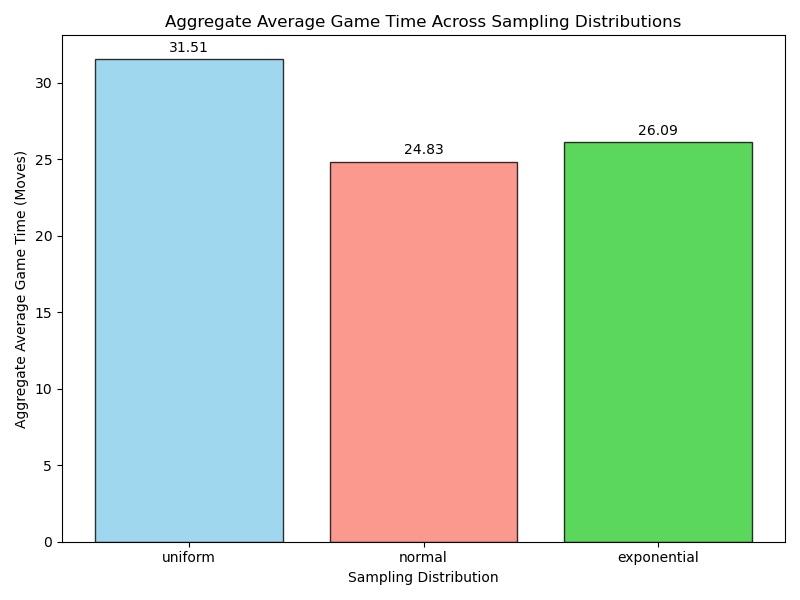
\includegraphics[width=0.5\textwidth]{"/home/ja1peg/Desktop/DissertationDocs/Dissertation/Chapter 2/withLength/FinalSampling/comparative_aggregate_average_game_times.png"} 
	\caption{\textbf{Aggregated Averages of Game Duration across the sampling distributions:} Bar plot compares average game durations for uniform, normal, and exponential length distributions. Exponential distribution yields highest, Uniform distribution lowest average game duration, suggesting shorter lengths extend game duration.}
	\label{fig:sampling_dist_avg_times}
\end{figure}

\begin{figure}[ht]
	\centering
	\subfloat[]{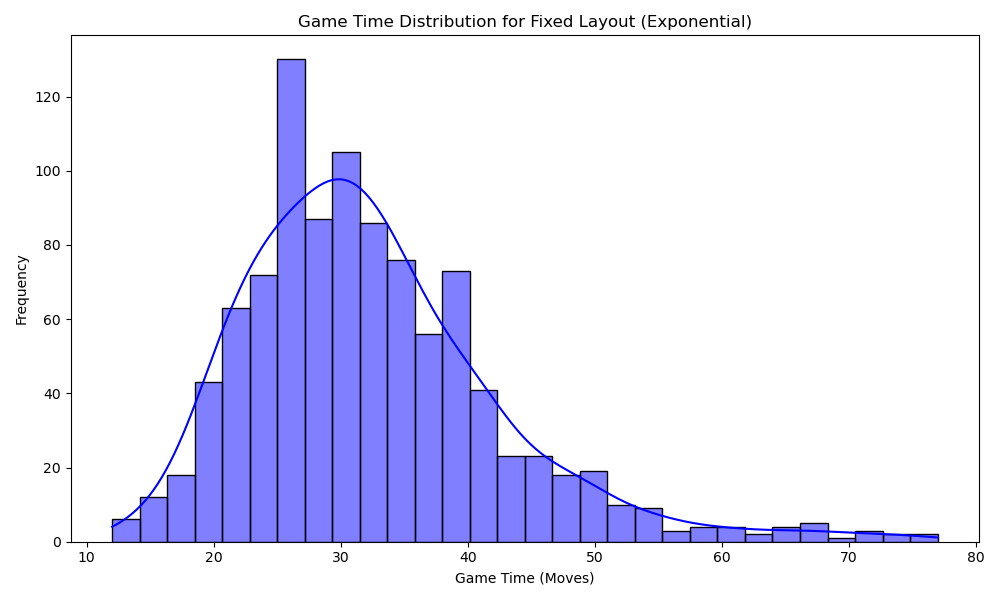
\includegraphics[width=0.5\textwidth]{"/home/ja1peg/Desktop/DissertationDocs/Dissertation/Chapter 2/withLength/FinalSampling/full_distribution_exponential.png"}} 
	\subfloat[]{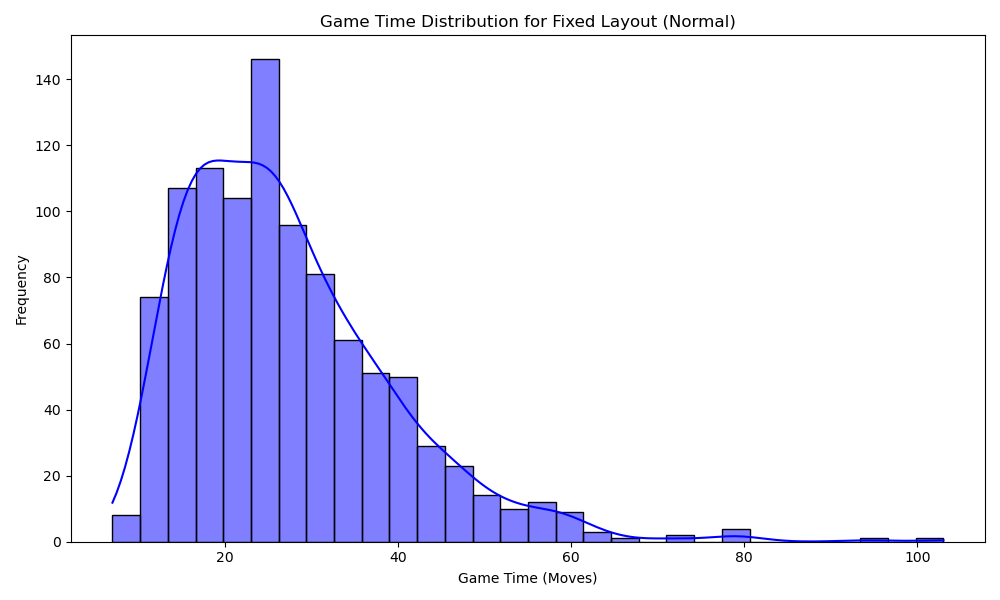
\includegraphics[width=0.5\textwidth]{"/home/ja1peg/Desktop/DissertationDocs/Dissertation/Chapter 2/withLength/FinalSampling/full_distribution_normal.png"}} 
	\linebreak
	\subfloat[]{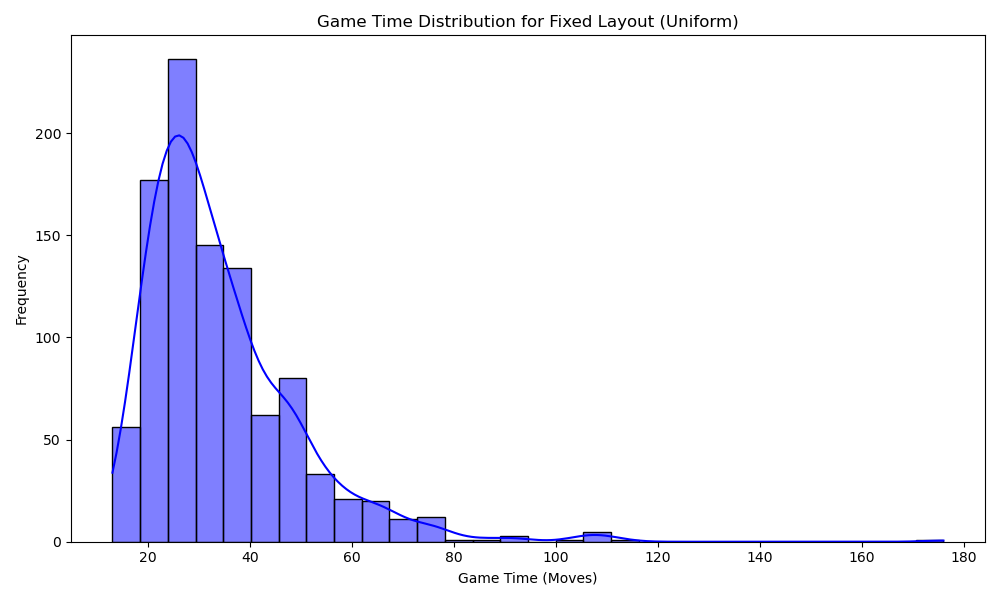
\includegraphics[width=0.5\textwidth]{/home/ja1peg/Desktop/DissertationDocs/Dissertation/Chapter 2/withLength/FinalSampling/full_distribution_uniform.png}} 
	\caption{\textbf{Game Durations Distributions for a Fixed Layout, by Sampling Method:} Histograms for a fixed layout show right-skewness across all sampling methods. Exponential sampling exhibits highest variability, possibly due to smaller entities and placement.}
	\label{fig:sampling_dist_layout_dists}
\end{figure}

Frequency distributions of game durations for a fixed board layout under each sampling method (Fig. \ref{fig:sampling_dist_layout_dists}) reveal right-skewness across all three distributions, indicating that while most games finish within a moderate set of moves, outliers leading to longer games are possible. Exponential sampling exhibits the largest outliers, due to the prevalence of smaller entities and their random placement. Figure \ref{fig:sampling_dist_board_avg_times} (a) indicates that boards generated using exponential sampling consistently result in higher average game durations compared to other methods. Figure \ref{fig:sampling_dist_board_avg_times} (b) shows that the normal distribution results in more consistently lower average game durations across different board layouts, albeit with some boards exhibiting higher averages. The Uniform distribution \ref{fig:sampling_dist_board_avg_times} (c) displays the most variability across the boards played.


\begin{figure}[ht]
	\centering
	\subfloat[]{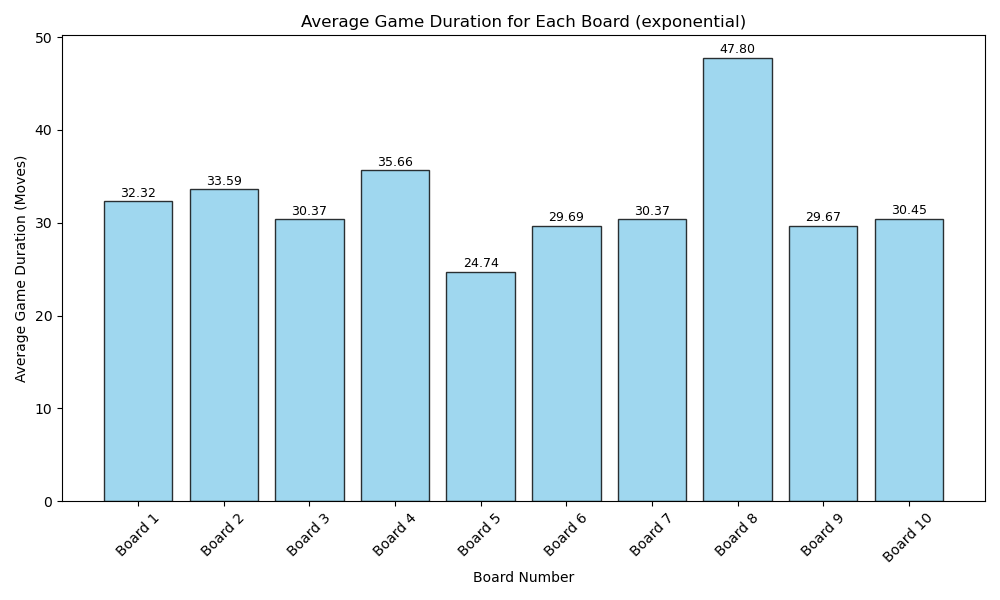
\includegraphics[width=0.45\textwidth]{"/home/ja1peg/Desktop/DissertationDocs/Dissertation/Chapter 2/withLength/FinalSampling/board_averages_exponential.png"}} 
	\subfloat[]{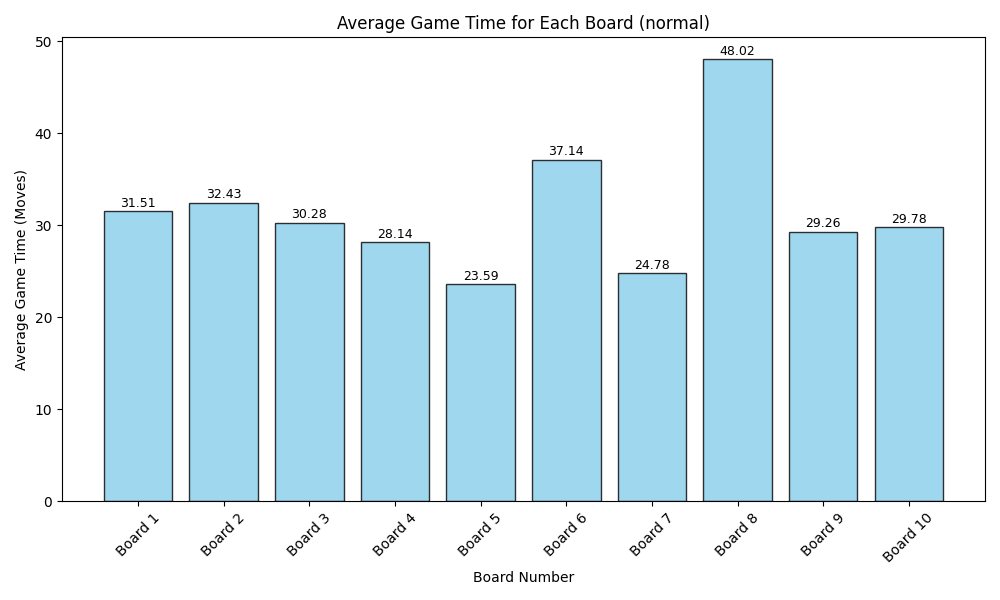
\includegraphics[width=0.45\textwidth]{"/home/ja1peg/Desktop/DissertationDocs/Dissertation/Chapter 2/withLength/FinalSampling/board_averages_normal.png"}}
	\linebreak
	\subfloat[]{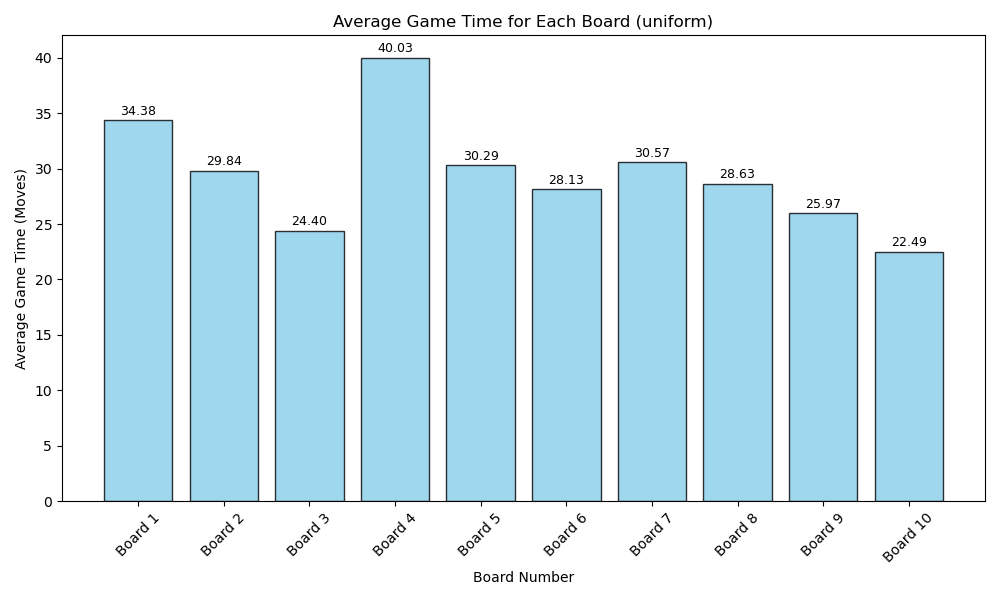
\includegraphics[width=0.45\textwidth]{"/home/ja1peg/Desktop/DissertationDocs/Dissertation/Chapter 2/withLength/FinalSampling/board_averages_uniform.png"}}
	\caption{\textbf{Average Game Duration for Each Board, by Sampling Distribution:} The plots show average game duration for 10 boards, by sampling distribution. Uniform distribution (c) yields consistently lower averages. Normal distribution (b) shows highest board variability, but low average times. Exponential sampling (a) generally results in higher average times.}
	\label{fig:sampling_dist_board_avg_times}
\end{figure}


\subsubsection{Fixed Start and End Points}

This section examines the effect of $L^s$ and $L^l$ being assigned randomly based on a fixed start and end position. Positions are generated while adhering to length constraints (i.e. the Snake and Ladder Constraints mentioned before and $L_{\text{max}} = 40$). This approach introduces greater variability compared to methods where lengths are predetermined because the lengths were being picked at random and can allow for certain board configurations to only have small $L^s$ and $L^l$ or conversely, it could lead to the average game duration falling down considerably due to larger entities. Figure \ref{fig:random_boards_avg_times} (b) illustrates average game durations across all 10 boards that were generated. Each bar represents the average game duration for a specific board, revealing significant variability in average game durations across different board layouts, ranging from approximately 22 to 55 moves. Figure \ref{fig:random_boards_game_dist} (a) displays the frequency distribution of game durations across all simulated games, indicating the right skewness of the approach to assigning lengths. Certain boards, due to their specific configurations, present varying challenges and opportunities for the agent, leading to a wide range of game durations.

\begin{figure}[ht]
	\centering
	\subfloat[]{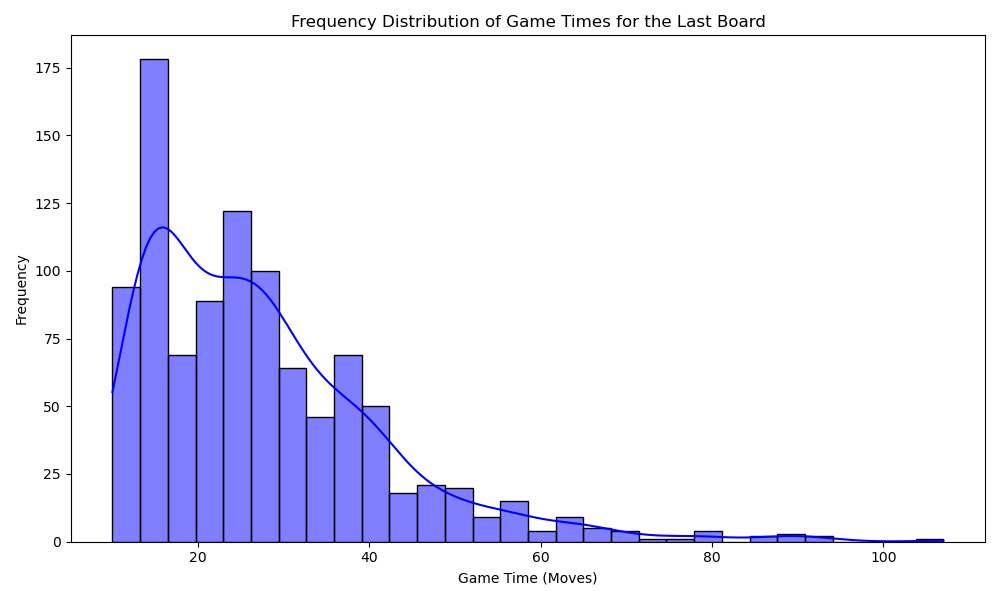
\includegraphics[width=0.45\textwidth]{"/home/ja1peg/Desktop/DissertationDocs/Dissertation/Chapter 2/withLength/RandomLength/approach_3_game_time_distribution.png"}}
	\subfloat[]{\includegraphics[width=0.45\textwidth]{"/home/ja1peg/Desktop/DissertationDocs/Dissertation/Chapter 2/withLength/RandomLength/approach\_3\_random\_points.png"}} 
	\linebreak
	\caption{\textbf{Analysis of Randomly Generated Boards:} (a) Game Duration distribution for the last board shows variability within a board. (b) Average game duration across 10 random boards varies significantly (22-55 moves), highlighting random placement impact.}
	\label{fig:random_boards_avg_times}
	\label{fig:random_boards_game_dist}
\end{figure}


\subsubsection{Insights from varying the lengths systematically}

This chapter explores the impacts of both entity $N_s$ and $N_l$ and, $L^S$ and $L^L$ on game duration in \textit{Snakes and Ladders}. By simulating games under systematically varied parameters through different approaches—static length assignment, statistical length sampling, and randomised start/end points, we obtained several insights.

Firstly, variations in both the \textit{number} and \textit{lengths} of snakes and ladders significantly influence game duration and its variability. Increased numbers of snakes generally prolong games, while more ladders tend to shorten them. However, the growth/decay in game duration with entity lengths is not always linear, with thresholds and interactions between entity types playing a crucial role. For example, while simply increasing snake count does not always linearly increase game duration, exceeding a certain density of snakes dramatically extends game duration. Conversely, the positive impact of ladders is more pronounced in mitigating the negative effects of high snake counts.

Secondly, the method of assigning entity lengths introduces another layer of complexity. Deterministic length assignments provide a baseline for understanding game mechanics, while statistical sampling reveals how different length distributions affect game variability and average duration. Exponential distributions, favouring shorter lengths, tend to increase game duration and variability, whereas normal distributions offer a more balanced outcome. Uniform distributions, in contrast, result in shorter, more predictable games. Randomly generated boards based on fixed start and end points introduce the highest degree of variability, highlighting the significant impact of entity placement on overall game dynamics.

Thirdly, the presence of outliers and fluctuating trend lines across different board layouts underscores the significant influence of board layout itself. Strategic placement of snakes and ladders can create ``traps" or ``shortcuts," leading to substantial variations in game duration even within the same parameter configurations.

These insights demonstrate how adjusting the number and lengths of snakes and ladders can fine-tune game difficulty and duration. The choice of length assignment method—deterministic, sampled, or position-based—further allows designers to control the level of variability and unpredictability in gameplay. For games with mechanics similar to \textit{Snakes and Ladders}, these insights can inform the creation of engaging experiences with carefully calibrated challenge and playtime.

Additionally, this chapter's exploration of entity number and length, while illuminating, represents just one facet of game design parametrisation. The observed sensitivity of game dynamics to these entity-level adjustments naturally prompts further investigation into other fundamental game design elements. In the subsequent chapter, we pivot our focus to another core parameter: the \textit{scale} of the game board itself. By systematically varying board dimensions, while holding entity characteristics constant, we aim to unravel how board size, as a determinant of game space and traversal distance, independently shapes game hardness/difficulty, through game duration, and overall player experience. This shift in focus, from entity-level parameters to board-level dimensions, represents the next logical step in our systematic parametrisation of Snakes and Ladders gameplay, allowing for a more holistic understanding of the game's design space.
